% ======================================================
% writeup_architecture.tex
% Compiler: pdflatex (or xelatex)
% ======================================================
\documentclass[11pt]{article}
\usepackage{amsmath, amssymb, bm}
<<<<<<< HEAD
\usepackage{graphicx}
\usepackage[margin=2cm]{geometry}

\newcommand{\T}{^{T}}
=======
\usepackage[margin=2cm]{geometry}

\newcommand{\T}{^{\top}}
>>>>>>> test/qr-paper-reference
\newcommand{\lc}{\lambda_c}
\newcommand{\Ts}{T_s}
\newcommand{\kB}{k_B}


\begin{document}

<<<<<<< HEAD
=======
\noindent Positioning\_kf\_a
\vspace{0.5em}

>>>>>>> test/qr-paper-reference
% =====================================================================
\section{Plant and Control Law}
% =====================================================================

<<<<<<< HEAD
\subsection*{1.1\quad Continuous-time plant}

\begin{equation}
\gamma(x)\,\dot{x} \;=\; f_{dx} + f_{Dx} + f_T
\end{equation}

\subsection*{1.2\quad Discrete-time plant (zero-order hold)}

\begin{align}
a_x[k]     &\equiv \Delta t \,/\, \gamma(x[k]) \\[2pt]
x_D[k]     &\equiv a_x[k]\,f_{Dx}[k] \\[2pt]
x[k\!+\!1] &= x[k] + a_x[k]\bigl(f_{dx}[k] + f_T[k]\bigr) + x_D[k]
\end{align}

\subsection*{1.3\quad Thermal force statistics}

$f_T[k]$ is zero-mean Gaussian white with variance
\begin{equation}
\sigma^{2}_{f_T}[k] \;=\; \frac{4\kB T\,\gamma(x[k])}{\Delta t}
\quad\Longrightarrow\quad
\mathrm{Var}\bigl(a_x[k]\,f_T[k]\bigr) \;=\; 4\kB T\,a_x[k].
\end{equation}

\subsection*{1.4\quad Control law}

\begin{equation}
f_{dx}[k] \;=\; \hat{a}_x^{-1}[k]\Bigl[\bigl(x_d[k\!+\!1] - x_d[k]\bigr)
  + (1-\lc)\,\delta\hat{x}[k] - \hat{x}_D[k]\Bigr]
\end{equation}

\noindent In the augmented state of \S3, $\delta\hat{x}[k] = \delta\hat{x}_3[k]$ (due to the two-step measurement delay; see \S3).

=======
\begin{align}
\gamma(x)\,\dot{x} &= f_{dx} + f_T \\[2pt]
a_x[k] &\equiv \Ts \,/\, \gamma(x[k]) \\[2pt]
x[k\!+\!1] &= x[k] + a_x[k]\bigl(f_{dx}[k] + f_T[k]\bigr),
  \qquad \mathrm{Var}\bigl(a_x[k]\,f_T[k]\bigr) = 4\kB T\,a_x[k] \\[4pt]
f_{dx}[k] &= \frac{1}{\hat{a}_x[k]}\Bigl[\bigl(x_d[k\!+\!1] - x_d[k]\bigr)
  + (1-\lc)\,\delta\hat{x}_3[k] - \hat{x}_D[k]\Bigr]
\end{align}

>>>>>>> test/qr-paper-reference
% =====================================================================
\section{IIR Variance Estimator for $a_x[k]$}
% =====================================================================

<<<<<<< HEAD
This section details the infinite impulse response (IIR) variance estimator that produces the auxiliary measurement $a_{xm}$ from the measured tracking error. The pipeline combines low-pass (LP) and high-pass (HP) stages.

\subsection*{2.1\quad Tracking error and high-pass filter}

\begin{align}
\delta x_m[k]    &= x_d[k\!-\!2] - x_m[k] \\[2pt]
\delta x_{md}[k] &= (1-a_{pd})\,\delta x_{md}[k\!-\!1] + a_{pd}\,\delta x_m[k] \\[2pt]
\delta x_{mr}[k] &= \delta x_m[k] - \delta x_{md}[k]
\end{align}

\noindent Only $\delta x_{mr}$ is driven by $a_x\,f_T$; $\delta x_{md}$ holds the trajectory-tracking mean.

\subsection*{2.2\quad Single-sample variance estimator}

$\sigma^{2}(X) = \mathrm{E}[X^{2}] - (\mathrm{E}[X])^{2}$ with two IIR sub-estimators:
\begin{align}
\delta x_{mrd}[k]                  &= (1-a_{prd})\,\delta x_{mrd}[k\!-\!1] + a_{prd}\,\delta x_{mr}[k] \\[2pt]
\overline{(\delta x_{mr})^{2}}[k]  &= (1-a_{cov})\,\overline{(\delta x_{mr})^{2}}[k\!-\!1]
  + a_{cov}\,\bigl(\delta x_{mr}[k]\bigr)^{2} \\[2pt]
\sigma^{2}_{\delta x_{mr}}[k]      &= \overline{(\delta x_{mr})^{2}}[k] - \bigl(\delta x_{mrd}[k]\bigr)^{2}
\end{align}

\subsection*{2.3\quad Role of the three IIR coefficients}

\begin{center}
\begin{tabular}{l l l}
\hline
coef & role & analyzed in \\
\hline
$a_{pd}$  & LP pole of $\delta x_m$; defines $\delta x_{mr}$ & \S5 ($C_{\mathrm{dpmr}}, C_n$) \\
$a_{prd}$ & LP pole of $\delta x_{mr}$                       & \S6 ($\beta$) \\
$a_{cov}$ & LP pole of $\overline{(\delta x_{mr})^{2}}$      & bias-free; estimator variance only \\
\hline
\end{tabular}
\end{center}

\subsection*{2.4\quad Link between $\sigma^{2}_{\delta x_{mr}}$ and $a_x$}

\begin{equation}
\boxed{\;\;
\sigma^{2}_{\delta x_{mr}}[k] \;\approx\; \beta\,\bigl(C_{\mathrm{dpmr}}\cdot 4\kB T\,a_x[k] + C_{n}\,\sigma^{2}_n\bigr)
\;\;}
\end{equation}

\noindent $(C_{\mathrm{dpmr}}, C_n)$ derived in \S5; $\beta$ in \S6.
\begin{equation}
a_{xm}[k] \;=\; \frac{\sigma^{2}_{\delta x_{mr}}[k]/\beta \,-\, C_{n}\,\sigma^{2}_n}
                    {C_{\mathrm{dpmr}}\cdot 4\kB T}
\end{equation}

% =====================================================================
\section{Kalman Filter (KF)}
% =====================================================================

\subsection*{3.1\quad State vector and process model}

\begin{align}
\bm{x}[k]      &= \bigl[\,\delta x_1,\;\delta x_2,\;\delta x_3,\;
  x_D,\;\delta x_D,\;a_x,\;\delta a_x\,\bigr]\T[k] \\[2pt]
\bm{x}[k\!+\!1] &= \bm{F}_{e}\,\bm{x}[k] + \bm{q}[k]
\end{align}

\[
\bm{F}_{e} =
=======
\begin{align}
\delta x_m[k] &= x_d[k\!-\!2] - x_m[k] \\[2pt]
\delta x_{md}[k] &= (1-a_{pd})\,\delta x_{md}[k\!-\!1] + a_{pd}\,\delta x_m[k] \\[2pt]
\delta x_{mr}[k] &= \delta x_m[k] - \delta x_{md}[k] \\[2pt]
\delta x_{mrd}[k] &= (1-a_{prd})\,\delta x_{mrd}[k\!-\!1] + a_{prd}\,\delta x_{mr}[k] \\[2pt]
\overline{(\delta x_{mr})^{2}}[k] &= (1-a_{cov})\,\overline{(\delta x_{mr})^{2}}[k\!-\!1]
  + a_{cov}\,\bigl(\delta x_{mr}[k]\bigr)^{2} \\[2pt]
\sigma^{2}_{\delta x_{mr}}[k] &= \overline{(\delta x_{mr})^{2}}[k]
  - \bigl(\delta x_{mrd}[k]\bigr)^{2} \\[4pt]
\sigma^{2}_{\delta x_{mr}}[k] &= C_{\mathrm{dpmr}}\cdot 4\kB T\,a_x[k]
  \;+\; C_{n}\,\sigma^{2}_n \\[4pt]
\boxed{\;\;
a_{xm}[k] \;=\; \dfrac{\sigma^{2}_{\delta x_{mr}}[k] - C_{n}\,\sigma^{2}_n}
                    {C_{\mathrm{dpmr}}\cdot 4\kB T}
\;\;}
\end{align}

% =====================================================================
\section{Kalman Filter}
% =====================================================================

\begin{align}
\bm{x}[k] &= \bigl[\,\delta x_1,\;\delta x_2,\;\delta x_3,\;
  x_D,\;\delta x_D,\;a_x,\;\delta a_x\,\bigr]\T[k] \\[4pt]
\bm{x}[k\!+\!1] &= \bm{F}_{e}\,\bm{x}[k] + \bm{q}[k],
  \qquad
  \bm{y}[k] = \bm{H}\,\bm{x}[k] + \bm{v}[k]
  = \begin{bmatrix}\delta x_m[k]\\[2pt] a_{xm}[k]\end{bmatrix} \\[6pt]
\bm{F}_{e} &=
>>>>>>> test/qr-paper-reference
\begin{bmatrix}
  0 & 1 & 0 & 0 & 0 & 0 & 0 \\
  0 & 0 & 1 & 0 & 0 & 0 & 0 \\
  0 & 0 & 1 & -1 & 0 & -f_{dx}[k] & 0 \\
  0 & 0 & 0 & 1 & 1 & 0 & 0 \\
  0 & 0 & 0 & 0 & 1 & 0 & 0 \\
  0 & 0 & 0 & 0 & 0 & 1 & 1 \\
  0 & 0 & 0 & 0 & 0 & 0 & 1
<<<<<<< HEAD
\end{bmatrix}
\]

\subsection*{3.2\quad Measurement model}

\begin{equation}
\bm{y}[k] = \bm{H}\,\bm{x}[k] + \bm{v}[k]
  = \begin{bmatrix}\delta x_m[k]\\[2pt] a_{xm}[k]\end{bmatrix}
\end{equation}

\[
=======
\end{bmatrix},
\qquad
>>>>>>> test/qr-paper-reference
\bm{H} =
\begin{bmatrix}
  1 & 0 & 0 & 0 & 0 & 0 & 0 \\
  0 & 0 & 0 & 0 & 0 & 1 & 0
<<<<<<< HEAD
\end{bmatrix}
\]

\subsection*{3.3\quad Kalman filter recursions}

\begin{align}
\bm{L}[k]                  &= \bm{P}_f[k]\,\bm{H}\T\bigl(\bm{H}\,\bm{P}_f[k]\,\bm{H}\T + \bm{R}\bigr)^{-1} \\[2pt]
\bm{P}[k]                  &= (\bm{I} - \bm{L}[k]\,\bm{H})\,\bm{P}_f[k] \\[2pt]
\bm{P}_f[k\!+\!1]          &= \bm{F}_{e}\,\bm{P}[k]\,\bm{F}_{e}\T + \bm{Q} \\[2pt]
=======
\end{bmatrix} \\[6pt]
\bm{L}[k] &= \bm{P}'[k]\,\bm{H}\T\bigl(\bm{H}\,\bm{P}'[k]\,\bm{H}\T + \bm{R}\bigr)^{-1} \\[2pt]
\bm{P}[k] &= (\bm{I} - \bm{L}[k]\,\bm{H})\,\bm{P}'[k] \\[2pt]
\bm{P}'[k\!+\!1] &= \bm{F}_{e}\,\bm{P}[k]\,\bm{F}_{e}\T + \bm{Q} \\[4pt]
>>>>>>> test/qr-paper-reference
\hat{\bm{x}}[k\!+\!1\,|\,k] &= \bm{F}_{e}\,\hat{\bm{x}}[k\,|\,k\!-\!1]
  + \bm{F}_{e}\,\bm{L}_{ss}\bigl(\bm{y}[k] - \bm{H}\,\hat{\bm{x}}[k\,|\,k\!-\!1]\bigr)
\end{align}

<<<<<<< HEAD
\setcounter{section}{4}
=======
All three axes use the same $\bm{F}_e$ above (random-walk Jordan blocks
for the disturbance and motion-gain state pairs).

% =====================================================================
\section{Simulation Setup}
% =====================================================================

\begin{align}
h_{\mathrm{init}} &\in \{50,\ 2.5\}\ \mu\mathrm{m},
  \qquad \sigma^{2}_n = 0 \\[2pt]
\lc &= 0.7,
  \qquad a_{pd} = a_{prd} = a_{cov} = 0.05 \\[4pt]
\hat{a}[0] &= \Bigl[\;
  \tfrac{a_{\mathrm{nom}}}{c_{\parallel}(h_{\mathrm{init}}/R)},\;
  \tfrac{a_{\mathrm{nom}}}{c_{\parallel}(h_{\mathrm{init}}/R)},\;
  \tfrac{a_{\mathrm{nom}}}{c_{\perp}(h_{\mathrm{init}}/R)}
\;\Bigr]\T,
  \qquad a_{\mathrm{nom}} \equiv \Ts / \gamma_N \\[6pt]
\bm{Q} &= \frac{4\kB T\,\Ts}{\gamma_N}\cdot
\begin{bmatrix}
  0 & 0 & 0 & 0 & 0 & 0 & 0 \\
  0 & 0 & 0 & 0 & 0 & 0 & 0 \\
  0 & 0 & 10^{4} & 0 & 0 & 0 & 0 \\
  0 & 0 & 0 & 10^{-1} & 0 & 0 & 0 \\
  0 & 0 & 0 & 0 & 0 & 0 & 0 \\
  0 & 0 & 0 & 0 & 0 & 10^{-4} & 0 \\
  0 & 0 & 0 & 0 & 0 & 0 & 0
\end{bmatrix} \\[6pt]
\bm{R} &= \frac{4\kB T\,\Ts}{\gamma_N}\cdot
\begin{bmatrix}
  10^{-2} & 0 \\[2pt]
  0 & 10^{0}
\end{bmatrix}
\end{align}

\begin{align*}
h = 50\ \mu\mathrm{m}:\ &\quad c_\perp \approx 1.05,
  \quad a_{\mathrm{true}} \approx a_{\mathrm{nom}} \\
h = 2.5\ \mu\mathrm{m}:\ &\quad c_\perp \approx 10.4,
  \quad a_{\mathrm{true}} \approx 0.10\,a_{\mathrm{nom}}
\end{align*}
>>>>>>> test/qr-paper-reference

% =====================================================================
\section{Closed-Loop Steady-State Variance: $C_{\mathrm{dpmr}}$ and $C_{n}$}
% =====================================================================

<<<<<<< HEAD
\emph{Scope note.} The derivation drops the time-varying entry $\bm{F}_e(3,6) = -f_{dx}[k]$ from the $\bm{A}$ matrix to obtain a time-invariant system so that Lyapunov analysis applies. Under zero-mean $f_{dx}$ operating conditions (static regulation with $\Delta p_d = 0$, or symmetric oscillatory reference), the dropped $f_{dx}\!\cdot\!e_a$ term has $\mathrm{E}[f_{dx}\!\cdot\!e_a] \approx 0$ and contributes variance of order $\sigma^{2}_{f}\sigma^{2}_{e}$, which is negligible relative to the dominant thermal term $4\kB T\,a_x$ (i.e.\ $\sigma^{2}_{f}\sigma^{2}_{e} / (4\kB T\,a_x) \ll 1$). Empirical variance matches the derived $C_{\mathrm{dpmr}}$ at all operating points tested (free-space, near-wall static, dynamic sweep).

\subsection*{5.1\quad Augmented state and closed-loop dynamics}
=======
\emph{Scope note.} This section derives $C_{\mathrm{dpmr}}$ and $C_n$
using one linearization simplification: the $f_{dx}[k]$ sensitivity
entry $\bm{F}_e(3,6) = -f_{dx}[k]$ is treated as a small zero-mean
contribution and dropped, equivalent to setting $f_{dx} \!\to\! 0$ in
the Riccati solve. This is accurate at the free-space operating point
($h \!\gg\! R$, $c_\perp \!\approx\! 1$), where empirical variance
matches the derived $C_{\mathrm{dpmr}}$ within $\pm 2\%$ (Task P2 report).
The behavior at extreme near-wall is quantified in the same report.

\subsection*{5.1\quad Augmented state}
>>>>>>> test/qr-paper-reference

\[
\bm{e}[k] \;=\; \bigl[\,
  \delta x_1,\; \delta x_2,\; \delta x_3,\;\;
  e_{x1},\; e_{x2},\; e_{x3},\;\;
  e_{xD},\; e_{\delta xD},\; e_{a},\; e_{\delta a},\;\;
  \delta x_{md}[k\!-\!1]
\,\bigr]\T[k]
\;\in\; \mathbb{R}^{11}
\]

<<<<<<< HEAD
=======


\subsection*{5.2\quad Closed-loop recursion for $\delta x_3$}

Plant $+$ Section 1 control law (fluctuation frame, $x_D\!=\!0$, $\hat{a}_x \!\approx\! a_x$; $f_{dx}$ sensitivity dropped per §5 scope note):

\begin{equation}
\delta x_3[k\!+\!1] \;=\; \lc\,\delta x_3[k]
   \;+\; (1{-}\lc)\,e_{x3}[k]
   \;-\; e_{xD}[k]
   \;-\; a_x[k]\,f_T[k]
\end{equation}

\subsection*{5.3\quad Augmented dynamics}

>>>>>>> test/qr-paper-reference
\begin{equation}
\bm{e}[k\!+\!1] \;=\; \bm{A}\,\bm{e}[k]
  \;+\; \bm{b}_T\bigl(a_x[k]\,f_T[k]\bigr)
  \;+\; \bm{b}_n\,n[k]
\end{equation}

<<<<<<< HEAD
=======


>>>>>>> test/qr-paper-reference
\[
\bm{A} \;=\;
\left[\begin{array}{ccc|ccccccc|c}
0 & 1 & 0   & 0 & 0 & 0 & 0 & 0 & 0 & 0 & 0 \\
0 & 0 & 1   & 0 & 0 & 0 & 0 & 0 & 0 & 0 & 0 \\
0 & 0 & \lc & 0 & 0 & 1{-}\lc & {-}1 & 0 & 0 & 0 & 0 \\
\hline
\multicolumn{3}{c|}{\bm{0}_{7\times 3}} & \multicolumn{7}{c|}{\bm{A}_e} & \multicolumn{1}{c}{\bm{0}_{7\times 1}} \\
\hline
a_{pd} & 0 & 0 & 0 & 0 & 0 & 0 & 0 & 0 & 0 & 1{-}a_{pd}
\end{array}\right]
\]

<<<<<<< HEAD
\noindent where $\bm{A}_e \equiv \bm{F}_e(\bm{I} - \bm{L}_{ss}\bm{H})$ is the steady-state KF estimation-error dynamics (\S3.3).

=======
\noindent Noise vectors:
>>>>>>> test/qr-paper-reference
\[
\bm{b}_T \;=\; \bigl[\,0,\,0,\,{-}1,\;\;0,\,0,\,{-}1,\,0,\,0,\,0,\,0,\;\;0\,\bigr]\T,
\qquad
\bm{b}_n \;=\; \bigl[\,0,\,0,\,0,\;\;{-}\bm{F}_e\bm{L}_{ss}(:,1),\;\;{-}a_{pd}\,\bigr]\T
\]

<<<<<<< HEAD
\subsection*{5.2\quad Lyapunov decomposition}

Define $\bm{\Sigma}[k] \equiv \mathrm{E}\bigl[\bm{e}[k]\bm{e}[k]\T\bigr]$. Since $f_T[k]$ and $n[k]$ are independent zero-mean white processes, $\bm{\Sigma}$ decomposes linearly:
=======
\subsection*{5.4\quad Lyapunov decomposition and computation}

Define $\bm{\Sigma}[k] \!\equiv\! \mathrm{E}\bigl[\bm{e}[k]\bm{e}[k]\T\bigr]$.
Because $f_T[k]$ and $n[k]$ are independent zero-mean white processes,
>>>>>>> test/qr-paper-reference
\begin{align}
\bm{\Sigma}[k] &\;=\; 4\kB T\,a_x[k]\;\bm{\Sigma}_T \;+\; \sigma^{2}_n\;\bm{\Sigma}_n \\[2pt]
\bm{\Sigma}_T  &\;=\; \bm{A}\,\bm{\Sigma}_T\,\bm{A}\T \;+\; \bm{b}_T\,\bm{b}_T\T \\[2pt]
\bm{\Sigma}_n  &\;=\; \bm{A}\,\bm{\Sigma}_n\,\bm{A}\T \;+\; \bm{b}_n\,\bm{b}_n\T
\end{align}

<<<<<<< HEAD
\subsection*{5.3\quad Variance of $\delta x_{mr}$}

Substituting the \S2.1 LP recursion into the HP residual definition, with $\delta x_m[k] = \delta x_1[k] - n[k]$:
=======


\subsection*{5.5\quad Variance of $\delta x_{mr}$}

Inverting the Section 2 LP recursion, with $\delta x_m[k] = \delta x_1[k] - n[k]$:

>>>>>>> test/qr-paper-reference
\begin{equation}
\delta x_{mr}[k] \;=\; (1-a_{pd})\bigl(\delta x_1[k] - \delta x_{md}[k\!-\!1] - n[k]\bigr)
\end{equation}

<<<<<<< HEAD
Variance ($n[k]$ independent of $\bm{e}[k]$):
=======
\noindent Variance ($n[k]$ independent of $\bm{e}[k]$):

>>>>>>> test/qr-paper-reference
\begin{equation}
\sigma^{2}_{\delta x_{mr}}[k]
  \;=\; (1-a_{pd})^{2}\Bigl[\,
    (\bm{\Sigma}[k])_{1,1} \,-\, 2\,(\bm{\Sigma}[k])_{1,11} \,+\, (\bm{\Sigma}[k])_{11,11}
    \,+\, \sigma^{2}_n
  \,\Bigr]
\end{equation}

<<<<<<< HEAD
\subsection*{5.4\quad $C_{\mathrm{dpmr}}$ and $C_{n}$}

\noindent Substituting $\bm{\Sigma}[k] = 4\kB T\,a_x[k]\,\bm{\Sigma}_T + \sigma^{2}_n\,\bm{\Sigma}_n$ into the \S5.3 variance formula and matching against the target $\sigma^{2}_{\delta x_{mr}} = C_{\mathrm{dpmr}}\cdot 4\kB T\,a_x + C_{n}\,\sigma^{2}_n$:

$\bm{\Sigma}_T$ and $\bm{\Sigma}_n$ are the discrete Lyapunov solutions --- equivalently, geometric series in $\bm{A}$ --- driven by $\bm{b}_T$ and $\bm{b}_n$ respectively:
\begin{align*}
\bm{\Sigma}_T(\lambda_c, a_{pd};\, \bm{Q}, \bm{R})
  &\;=\; \sum_{k=0}^{\infty} \bm{A}^{k}\,\bm{b}_T\bm{b}_T\T\,(\bm{A}\T)^{k} \\[2pt]
\bm{\Sigma}_n(\lambda_c, a_{pd};\, \bm{Q}, \bm{R})
  &\;=\; \sum_{k=0}^{\infty} \bm{A}^{k}\,\bm{b}_n\bm{b}_n\T\,(\bm{A}\T)^{k}
\end{align*}

\noindent (solutions of $\bm{A}\bm{\Sigma}_T\bm{A}\T + \bm{b}_T\bm{b}_T\T = \bm{\Sigma}_T$ and $\bm{A}\bm{\Sigma}_n\bm{A}\T + \bm{b}_n\bm{b}_n\T = \bm{\Sigma}_n$; $\bm{A}, \bm{b}_T, \bm{b}_n$ constructed per \S5.1.)

Therefore:
\begin{gather}
\boxed{\;C_{\mathrm{dpmr}}(\lambda_c, a_{pd};\, \bm{Q}, \bm{R}) \;=\; (1-a_{pd})^{2}\bigl[\,
  (\bm{\Sigma}_T)_{1,1} \,-\, 2\,(\bm{\Sigma}_T)_{1,11} \,+\, (\bm{\Sigma}_T)_{11,11}\,\bigr]\;} \\[4pt]
\boxed{\;C_{n}(\lambda_c, a_{pd};\, \bm{Q}, \bm{R}) \;=\; (1-a_{pd})^{2}\bigl[\,
  (\bm{\Sigma}_n)_{1,1} \,-\, 2\,(\bm{\Sigma}_n)_{1,11} \,+\, (\bm{\Sigma}_n)_{11,11} \,+\, 1\,\bigr]\;}
\end{gather}

\noindent The $+1$ in $C_{n}$ captures the direct contribution of the current $n[k]$ via the explicit $-n$ term in \S5.3; the $(\bm{\Sigma}_n)$ selector captures past $n[k]$'s propagated through the state dynamics $\bm{e}[k]$. With $(\bm{Q}, \bm{R})$ fixed at design time, the LUT is built offline on a $(\lambda_c, a_{pd})$ grid:

\begin{center}
\begin{tabular}{@{}l@{}}
\texttt{for each $(\lambda_c,\, a_{pd})$ in design grid:} \\
\quad build $\bm{A}$ and $\bm{b}_n$ per \S5.1 from $(\lambda_c, a_{pd}; \bm{Q}, \bm{R}, \bm{H})$ \\
\quad $\bm{\Sigma}_T \;\leftarrow\; \mathrm{dlyap}(\bm{A},\, \bm{b}_T\bm{b}_T\T)$ \\
\quad $\bm{\Sigma}_n \;\leftarrow\; \mathrm{dlyap}(\bm{A},\, \bm{b}_n\bm{b}_n\T)$ \\
\quad $C_{\mathrm{dpmr}}[\lambda_c, a_{pd}] \;\leftarrow\; (1-a_{pd})^2\,[(\bm{\Sigma}_T)_{1,1} - 2(\bm{\Sigma}_T)_{1,11} + (\bm{\Sigma}_T)_{11,11}]$ \\
\quad $C_{n}[\lambda_c, a_{pd}] \;\leftarrow\; (1-a_{pd})^2\,[(\bm{\Sigma}_n)_{1,1} - 2(\bm{\Sigma}_n)_{1,11} + (\bm{\Sigma}_n)_{11,11} + 1]$ \\
\end{tabular}
\end{center}
=======
\subsection*{5.6\quad $C_{\mathrm{dpmr}}$ and $C_{n}$}

Substitute $\bm{\Sigma}[k] = 4\kB T\,a_x[k]\,\bm{\Sigma}_T + \sigma^{2}_n\,\bm{\Sigma}_n$ and match
$\sigma^{2}_{\delta x_{mr}} = C_{\mathrm{dpmr}}\!\cdot\! 4\kB T\,a_x + C_{n}\!\cdot\! \sigma^{2}_n$:

\begin{gather}
\boxed{\;C_{\mathrm{dpmr}} \;=\; (1-a_{pd})^{2}\bigl[\,
  (\bm{\Sigma}_T)_{1,1} \,-\, 2\,(\bm{\Sigma}_T)_{1,11} \,+\, (\bm{\Sigma}_T)_{11,11}
  \,\bigr]\;} \\[6pt]
\boxed{\;C_{n} \;=\; (1-a_{pd})^{2}\bigl[\,
  (\bm{\Sigma}_n)_{1,1} \,-\, 2\,(\bm{\Sigma}_n)_{1,11} \,+\, (\bm{\Sigma}_n)_{11,11}
  \,+\, 1
  \,\bigr]\;}
\end{gather}

The $+1$ in $C_{n}$ is the direct contribution of $n[k]$ to $\delta x_{mr}[k]$ (does not pass through $\bm{e}[k]$).
>>>>>>> test/qr-paper-reference

% =====================================================================
\section{IIR Finite-Sample Bias Factor $\beta$}
% =====================================================================

\subsection*{6.1\quad Bias source}

The Section 2 IIR algorithm computes
$\sigma^{2}_{\delta x_{mr}}[k] = \overline{(\delta x_{mr})^{2}}[k] - (\delta x_{mrd}[k])^{2}$.
In stationary steady state ($\delta x_{mr}$ zero-mean):
\begin{align}
\mathrm{E}\bigl[\,\overline{(\delta x_{mr})^{2}}\,\bigr] &\;=\; \mathrm{Var}(\delta x_{mr}) \\[2pt]
\mathrm{E}\bigl[\,(\delta x_{mrd})^{2}\,\bigr] &\;=\; \mathrm{Var}(\delta x_{mrd})
\end{align}
<<<<<<< HEAD
so the IIR output systematically underestimates $\mathrm{Var}(\delta x_{mr})$ by the amount $\mathrm{Var}(\delta x_{mrd}) > 0$. Define the bias factor $\beta$ as the ratio of the IIR estimator's expected output $\mathrm{E}[\sigma^{2}_{\delta x_{mr}}]$ to the true variance $\mathrm{Var}(\delta x_{mr})$:
=======
so the IIR output is biased low by $\mathrm{Var}(\delta x_{mrd}) > 0$. Define
>>>>>>> test/qr-paper-reference
\begin{equation}
\beta \;\equiv\; \frac{\mathrm{E}\!\bigl[\,\sigma^{2}_{\delta x_{mr}}\,\bigr]}{\mathrm{Var}(\delta x_{mr})}
       \;=\; 1 \;-\; \frac{\mathrm{Var}(\delta x_{mrd})}{\mathrm{Var}(\delta x_{mr})}
\end{equation}

<<<<<<< HEAD
\subsection*{6.2\quad $\mathrm{Var}(\delta x_{mr})$ and autocorrelation $\rho(L)$}

\noindent To evaluate $\beta$, we need the denominator $\mathrm{Var}(\delta x_{mr})$ and the temporal autocorrelation $\rho(L)$ used for the numerator.

For the noise-free case ($\sigma^{2}_n = 0$), \S5's selector form gives
\begin{equation}
\mathrm{Var}(\delta x_{mr}) \;=\; (1{-}a_{pd})^{2}\bigl[\,(\bm{\Sigma}_T)_{1,1} - 2(\bm{\Sigma}_T)_{1,11} + (\bm{\Sigma}_T)_{11,11}\,\bigr]\cdot 4\kB T\, a_x.
\end{equation}

The lag-$L$ autocorrelation is defined as
\begin{equation}
\rho(L) \;\equiv\; \mathrm{Cov}\bigl(\delta x_{mr}[k],\, \delta x_{mr}[k\!-\!L]\bigr) \,/\, \mathrm{Var}(\delta x_{mr}).
\end{equation}

Since $\bm{A}^{L}\bm{\Sigma}_T$ is the lag-$L$ cross-covariance of $\bm{e}[k]$, applying the same selector (the common $(1-a_{pd})^2$ and $4 k_B T\,a_x$ prefactors cancel in the ratio) yields
\begin{equation}
\rho(L) \;=\; \frac{(\bm{A}^{L}\bm{\Sigma}_T)_{1,1} - 2(\bm{A}^{L}\bm{\Sigma}_T)_{1,11} + (\bm{A}^{L}\bm{\Sigma}_T)_{11,11}}
                     {(\bm{\Sigma}_T)_{1,1} - 2(\bm{\Sigma}_T)_{1,11} + (\bm{\Sigma}_T)_{11,11}}.
=======
\subsection*{6.2\quad $\mathrm{Var}(\delta x_{mr})$ and $\rho(L)$ from Section 5}

For the noise-free case ($\sigma^{2}_n = 0$), Section 5's selector form gives
\begin{equation}
\mathrm{Var}(\delta x_{mr}) \;=\; (1{-}a_{pd})^{2}\bigl[\,(\bm{\Sigma}_T)_{1,1} - 2(\bm{\Sigma}_T)_{1,11} + (\bm{\Sigma}_T)_{11,11}\,\bigr]\cdot 4\kB T\, a_x
\end{equation}
The lag-$L$ autocorrelation
$\rho(L) \equiv \mathrm{Cov}(\delta x_{mr}[k], \delta x_{mr}[k\!-\!L]) / \mathrm{Var}(\delta x_{mr})$
follows from $\bm{A}^{L}\bm{\Sigma}_T$ via the same selector
(the $(1{-}a_{pd})^{2}$ and $4\kB T\, a_x$ prefactors cancel):
\begin{equation}
\rho(L) \;=\; \frac{(\bm{A}^{L}\bm{\Sigma}_T)_{1,1} - 2(\bm{A}^{L}\bm{\Sigma}_T)_{1,11} + (\bm{A}^{L}\bm{\Sigma}_T)_{11,11}}
                     {(\bm{\Sigma}_T)_{1,1} - 2(\bm{\Sigma}_T)_{1,11} + (\bm{\Sigma}_T)_{11,11}}
>>>>>>> test/qr-paper-reference
\end{equation}

\subsection*{6.3\quad $\mathrm{Var}(\delta x_{mrd})$ closed form}

<<<<<<< HEAD
Unrolling the \S2.2 LP recursion converts $\delta x_{mrd}[k]$ into an explicit weighted sum of past $\delta x_{mr}$, so that $\mathrm{Var}(\delta x_{mrd})$ can be expressed via $\rho(L)$:
=======
Unroll the Section 2 LP recursion:
>>>>>>> test/qr-paper-reference
\begin{equation}
\delta x_{mrd}[k] \;=\; a_{prd}\sum_{j=0}^{\infty}(1{-}a_{prd})^{j}\,\delta x_{mr}[k\!-\!j]
\end{equation}
Take variance, split diagonal $j\!=\!l$ from off-diagonal $j\!\neq\!l$, and use
$\sum_{j=0}^{\infty}(1{-}a_{prd})^{2j} = 1/\bigl[a_{prd}(2{-}a_{prd})\bigr]$:
\begin{equation}
\mathrm{Var}(\delta x_{mrd}) \;=\; \frac{a_{prd}}{2 - a_{prd}}\,\mathrm{Var}(\delta x_{mr})\,\Bigl[\,1 + 2\sum_{m=1}^{\infty}\rho(m)(1{-}a_{prd})^{m}\,\Bigr]
\end{equation}

<<<<<<< HEAD
\subsection*{6.4\quad Bias factor $\beta$}

Substituting the $\mathrm{Var}(\delta x_{mrd})$ expression into the $\beta$ definition:
\begin{equation}
\boxed{\;\beta(\lc, a_{pd}, a_{prd};\, \bm{Q}, \bm{R}) \;=\; 1 \;-\; \frac{a_{prd}}{2 - a_{prd}}\,\Bigl[\,1 + 2\sum_{m=1}^{\infty}\rho(m)(1{-}a_{prd})^{m}\,\Bigr]\;}
\end{equation}

\noindent The bracket is the \emph{autocorrelation amplification}: $=1$ for white $\delta x_{mr}$, $>\!1$ for positively-correlated.

% =====================================================================
\section{Q/R Design}
% =====================================================================

This section derives each non-zero entry of the Kalman filter (KF) process-noise $\bm{Q}$ and measurement-noise $\bm{R}$ from physical first principles.

\subsection*{7.1\quad Zero elements of $\bm{Q}$}

\noindent $Q(i,i)$ represents the process noise entering state $i$. Under \emph{positioning} (probe held at fixed $h_{\mathrm{init}}$), most states have no driver:

\begin{itemize}
\item $\delta x_1, \delta x_2$: past values of $\delta x_3$, shifted by delay.
\item $x_D, \delta x_D$: disturbance is modeled as zero ($x_D \equiv 0$).
\item $\delta a_x$: $a = a_{\mathrm{nom}}/c_{\mathrm{axis}}(\bar h)$ is constant at fixed $h$, so $\delta a \equiv 0$.
\end{itemize}

\noindent Only two entries are non-zero: $Q(3,3)$ (thermal force injection into $\delta x_3$) and $Q(6,6)$ (a small positive regularization value, see below).

\bigskip
\subsection*{7.2\quad Non-zero elements of $\bm{Q}$}

\noindent\textbf{$Q(3,3)$ --- thermal force injection.}

\smallskip
\noindent Per-axis thermal-force variance from the Einstein relation with wall-corrected drag:
\begin{equation}
\mathrm{Var}(f_{T,\mathrm{axis}}) \;=\; \frac{4 k_B T\,\gamma_N\,c_\mathrm{axis}(\bar h)}{\Delta t}.
\end{equation}
Multiplying by $a_\mathrm{axis}^2$ gives the thermal injection into $\delta x_3$:
\begin{equation}
\mathrm{Var}(a_\mathrm{axis}\, f_T) \;=\; 4 k_B T \cdot a_\mathrm{axis} \;=\; a_\mathrm{ratio}\cdot\sigma^2_\mathrm{dXT},
\end{equation}
with $\sigma^2_\mathrm{dXT} \equiv 4 k_B T\, a_\mathrm{nom}$, $a_\mathrm{nom} \equiv \Delta t/\gamma_N$, $a_\mathrm{ratio} \equiv a_\mathrm{axis}/a_\mathrm{nom}$. Hence
\begin{equation}
\boxed{\;Q(3,3) \;=\; a_\mathrm{ratio} \cdot \sigma^2_\mathrm{dXT}\;}
\end{equation}

\bigskip
\noindent\textbf{$Q(6,6)$ --- a small positive value $\epsilon$.}

\smallskip
\noindent Under positioning, $a$ is constant, so physically $Q(6,6) = 0$. But setting $Q(6,6) = 0$ together with $Q(7,7) = 0$ makes the filter assume $a$ never varies: the discrete algebraic Riccati equation (DARE) then solves to $\bm{L}_{ss}(6,:) = 0$, meaning the filter's gain on the $a_{xm}$ measurement is zero --- $a_{xm}$ gets ignored entirely. To prevent this, add a small positive floor:
\begin{equation}
Q(6,6) \;=\; \epsilon \cdot \sigma^2_\mathrm{dXT}, \qquad \epsilon \ll 1.
\end{equation}
This tells the filter to allow a tiny slow drift in $a$, restoring a small non-zero $\bm{L}_{ss}(6,:)$ so that $a_{xm}$ can slowly update $\hat a$. $\epsilon$ is chosen small enough to preserve the scalar Riccati approximation used in \S8.3.

\subsection*{7.3\quad Measurement noise $\bm{R}$ (per axis)}

\noindent\textbf{$R(1,1)$ --- sensor noise on $\delta x_m$.} The position measurement has per-axis sensor-noise variance $\sigma^2_{n,\mathrm{axis}}$. Normalizing by the thermal unit:
\begin{equation}
\boxed{\;R(1,1)_\mathrm{axis} \;=\; \sigma^2_{n,\mathrm{axis}} \,/\, \sigma^2_\mathrm{dXT}\;}
\end{equation}
Per-axis is essential because different axes' tracking algorithms have $\sigma_n$ values spanning orders of magnitude.

\noindent\textbf{$R(2,2)$ --- sampling noise on $a_{xm}$.}

\smallskip
\noindent $a_{xm}$ is not a direct measurement --- it is the output of the IIR variance estimator (\S2.4). Its finite-sample noise variance takes the form
\begin{equation}
\mathrm{Var}(n_a) \;=\; \chi_\mathrm{sq} \cdot \rho_a \cdot a_\mathrm{axis}^2,
\end{equation}
built from three factors:
\begin{itemize}
\item $\chi_\mathrm{sq} \equiv 2 a_{cov} / (2 - a_{cov})$: exponential moving average (EMA) finite-sample factor.
\item $\rho_a \equiv 1 + 2 \sum_{L \geq 1} \rho^2(L)\,(1-a_{cov})^L$: autocorrelation amplification factor ($\geq 1$).
\item $a_\mathrm{axis}^2$: signal scale ($a_{xm}$ scales with $a$).
\end{itemize}
The squared $\rho^2$ (vs.\ \S6.4's linear $\rho$) arises because the EMA acts on $(\delta x_{mr})^2$: Wick/Isserlis gives the lag-$L$ autocorrelation of the squared Gaussian process as $\rho^2(L)$.

The $\rho(L)$ used here has the same selector structure as \S6.2 but with $V_\mathrm{state} + \sigma^2_n$ in the denominator (\S6.2's form is the $\sigma^2_n = 0$ limit).

Normalizing by the thermal unit:
\begin{equation}
\boxed{\;R(2,2)_\mathrm{axis} \;=\; \chi_\mathrm{sq} \cdot \rho_{a,\mathrm{axis}} \cdot a_\mathrm{axis}^2 \,/\, \sigma^2_\mathrm{dXT}\;}
\end{equation}

\bigskip
\subsection*{7.4\quad Summary: $\bm{Q}$ and $\bm{R}$ as functions of inputs}

\begin{equation}
\boxed{\;Q(3,3)(\bar h) \;=\; a_\mathrm{ratio}(\bar h)\cdot\sigma^2_\mathrm{dXT}\;}
\end{equation}

\begin{equation}
\boxed{\;Q(6,6)(\epsilon) \;=\; \epsilon\cdot\sigma^2_\mathrm{dXT}\;}
\end{equation}

\begin{equation}
\boxed{\;R(1,1)_\mathrm{axis}\bigl(\sigma^2_{n,\mathrm{axis}}\bigr) \;=\; \sigma^2_{n,\mathrm{axis}}\,/\,\sigma^2_\mathrm{dXT}\;}
\end{equation}

\begin{equation}
\boxed{\;R(2,2)_\mathrm{axis}\bigl(\bar h,\,a_{cov},\,\rho_{a,\mathrm{axis}}\bigr) \;=\; \chi_\mathrm{sq}\cdot\rho_{a,\mathrm{axis}}\cdot a_\mathrm{axis}^2(\bar h)\,/\,\sigma^2_\mathrm{dXT}\;}
\end{equation}

\noindent \emph{Note on $\rho_{a,\mathrm{axis}}$ dependency}: via $\bm{A}_\mathrm{aug}$ and $\bm{\Sigma}_\mathrm{aug}$, $\rho_{a,\mathrm{axis}}$ itself is a function of $(\lambda_c,\, a_{pd},\, a_{cov},\, \bar h,\, \epsilon,\, \sigma^2_{n,\mathrm{axis}})$ via a self-consistent fixed point. Hence $R(2,2)_\mathrm{axis}$ ultimately depends on the same input set.

% =====================================================================
\section{Theoretical Performance}
% =====================================================================

Combining the Q/R design of \S7 with the augmented Lyapunov framework of \S5 gives closed-form predictions for the tracking-error variance and the motion-gain estimation variance per axis.

\subsection*{8.1\quad Three-channel augmented covariance}

The two-channel decomposition of \S5.2 is extended with a third channel for the $a_{xm}$ sampling noise. Since $f_T$, $n_p$, and $n_a$ are mutually independent white noises, the augmented covariance splits linearly:
\begin{equation}
\boxed{\;\bm{\Sigma}_\mathrm{aug} \;=\; a_\mathrm{ratio}\,\sigma^2_\mathrm{dXT}\,\bm{\Sigma}_T
\;+\; \sigma^2_n\,\bm{\Sigma}_n
\;+\; \chi_\mathrm{sq}\,\rho_a\,a^2\,\bm{\Sigma}_{na}\;}
\end{equation}
Each $\bm{\Sigma}_X$ solves the unit-variance Lyapunov equation $\bm{\Sigma}_X = \bm{A}\,\bm{\Sigma}_X\,\bm{A}\T + \bm{b}_X\,\bm{b}_X\T$ with input vector
\begin{align*}
\bm{b}_T    &\;=\; \bigl[\,0,0,-1;\; 0,0,-1,0,0,0,0;\; 0\,\bigr]\T
  && \text{(thermal; \S5.1)} \\[2pt]
\bm{b}_n    &\;=\; \bigl[\,0,0,0;\; -\bm{F}_e\bm{L}_{ss}(:,1);\; -a_{pd}\,\bigr]\T
  && \text{(sensor; \S5.1)} \\[2pt]
\bm{b}_{na} &\;=\; \bigl[\,0,0,0;\; -\bm{F}_e\bm{L}_{ss}(:,2);\; 0\,\bigr]\T
  && \text{(new: $a_{xm}$ channel)}
\end{align*}
$\bm{b}_{na}$ mirrors $\bm{b}_n$ but uses the second column of $\bm{L}_{ss}$ (corresponding to the $a_{xm}$ measurement) and has a zero IIR entry because $a_{xm}$ does not feed the $\delta x_{md}$ filter.

\subsection*{8.2\quad Tracking-error variance (per axis)}

The first diagonal element of $\bm{\Sigma}_\mathrm{aug}$ (corresponding to $\delta x_1$, the tracking error) gives
\begin{equation}
\boxed{\;\mathrm{Var}(\delta x_\mathrm{axis}) \;=\; (\bm{\Sigma}_\mathrm{aug})_{1,1}\;}
\end{equation}
with three additive contributions:
\begin{itemize}\itemsep0pt
\item thermal: $a_\mathrm{ratio}\,\sigma^2_\mathrm{dXT}\,(\bm{\Sigma}_T)_{1,1}$
\item sensor: $\sigma^2_n\,(\bm{\Sigma}_n)_{1,1}$
\item $a_{xm}$ sampling: $\chi_\mathrm{sq}\,\rho_a\,a^2\,(\bm{\Sigma}_{na})_{1,1}$
\end{itemize}
Per-axis scaling enters through $a_\mathrm{ratio}$, $\sigma^2_{n,\mathrm{axis}}$, $a_\mathrm{axis}$, and $\rho_{a,\mathrm{axis}}$.

\subsection*{8.3\quad Motion-gain estimation (per axis)}

\noindent We evaluate the \emph{coefficient of variation} (CV) of the motion-gain estimate per axis:
\begin{equation}
\mathrm{CV}(\hat a_\mathrm{axis}) \;\equiv\; \mathrm{std}(\hat a_\mathrm{axis} - a_\mathrm{axis}) \,/\, a_\mathrm{axis}.
\end{equation}
$\mathrm{CV}^2$ is additive across independent noise sources. Two sources contribute here:
\begin{itemize}
\item \textbf{KF estimation error}: the KF cannot perfectly track $a$ from noisy $a_m$.
\item \textbf{Wall-effect on $a_\mathrm{true}$}: $a_\mathrm{true}(\bar h)$ itself varies as $\bar h$ fluctuates with the probe's $z$-error $\delta p_z$; independent of KF.
\end{itemize}
\noindent (Here $c_\mathrm{axis}$ denotes $c_\parallel$ for $x, y$ axes or $c_\perp$ for the $z$ axis, as defined in \S7.2.)
Thus
\begin{equation}
\mathrm{CV}^2(\hat a_\mathrm{axis}) \;=\; \mathrm{CV}^2_\mathrm{KF} \;+\; \mathrm{CV}^2_\mathrm{wall}.
\end{equation}

\bigskip
\noindent\textbf{Block A: KF estimation term.}

\smallskip
\noindent \textit{Step 1 --- Decoupling.} $Q(7,7) = 0$ (\S7.1) decouples the $(a, \delta a)$ KF block; the $a$-subsystem reduces to a scalar KF tracking $a$ from noisy $a_m$.

\smallskip
\noindent \textit{Step 2 --- Scalar Riccati gain.} The scalar discrete algebraic Riccati equation yields
\begin{equation}
L_\mathrm{eff,\,axis} \;=\; \sqrt{Q(6,6) \,/\, R(2,2)_\mathrm{axis}}.
\end{equation}
($L_\mathrm{eff}$ matches the full DARE gain $\bm{L}_{ss}(6,2)$ when $Q(7,7) = 0$; the approximation breaks at $Q(7,7) > 0$.)

\smallskip
\noindent \textit{Step 3 --- Input noise characterization.} The KF sees $a_m = a + n_a$ with $\mathrm{Var}(n_a) = \chi_\mathrm{sq}\,\rho_a\,a_\mathrm{axis}^2$ (\S7.3). Importantly, $n_a$ is a first-order autoregressive process (AR(1)) with bandwidth $a_{cov}$, inherited from the IIR EMA.

\smallskip
\noindent \textit{Step 4 --- Cascaded LP.} The KF (bandwidth $L_\mathrm{eff}$) low-passes the AR(1) noise $n_a$ (bandwidth $a_{cov}$). A two-state variance analysis (equivalent to integrating the cascaded AR(1) transfer function in the frequency domain) gives, in the small-$L_\mathrm{eff}$ and small-$a_{cov}$ limit:
\begin{equation}
\mathrm{Var}(\hat a - a) \,/\, \mathrm{Var}(n_a) \;=\; L_\mathrm{eff} \,/\, (L_\mathrm{eff} + a_{cov}).
\end{equation}
This replaces the standard $L_\mathrm{eff}/2$ result that would apply if $n_a$ were white noise.

\smallskip
\noindent Combining Step 3 and Step 4:
\begin{equation}
\boxed{\;\mathrm{CV}^2_\mathrm{KF,\,axis} \;=\; \chi_\mathrm{sq} \cdot \rho_{a,\mathrm{axis}} \cdot \frac{L_\mathrm{eff,\,axis}}{L_\mathrm{eff,\,axis} + a_{cov}}\;}
\end{equation}

\bigskip
\noindent\textbf{Block B: Wall-effect on $a_\mathrm{true}$.}

\smallskip
\noindent $a_\mathrm{true}(\bar h) = a_\mathrm{nom}/c_\mathrm{axis}(\bar h)$ depends on wall distance. Since $\delta \bar h = \delta p_z / R$ (up to sign), linearizing gives:
\begin{equation}
\boxed{\;\mathrm{CV}^2_\mathrm{wall,\,axis} \;=\; \left(\frac{|dc_\mathrm{axis}/d\bar h|}{c_\mathrm{axis}}\right)^{\!2} \cdot \frac{\mathrm{Var}(\delta p_z)}{R^2}\;}
\end{equation}

\bigskip
\noindent\textbf{Total (assuming independence):}
\begin{equation}
\boxed{\;\mathrm{CV}^2(\hat a_\mathrm{axis}) \;=\; \chi_\mathrm{sq}\,\rho_{a,\mathrm{axis}}\,\frac{L_\mathrm{eff}}{L_\mathrm{eff} + a_{cov}}
\;+\; \left(\frac{|dc_\mathrm{axis}/d\bar h|}{c_\mathrm{axis}}\right)^{\!2}\frac{\mathrm{Var}(\delta p_z)}{R^2}\;}
\end{equation}

\clearpage
\begin{figure}[p]
\centering
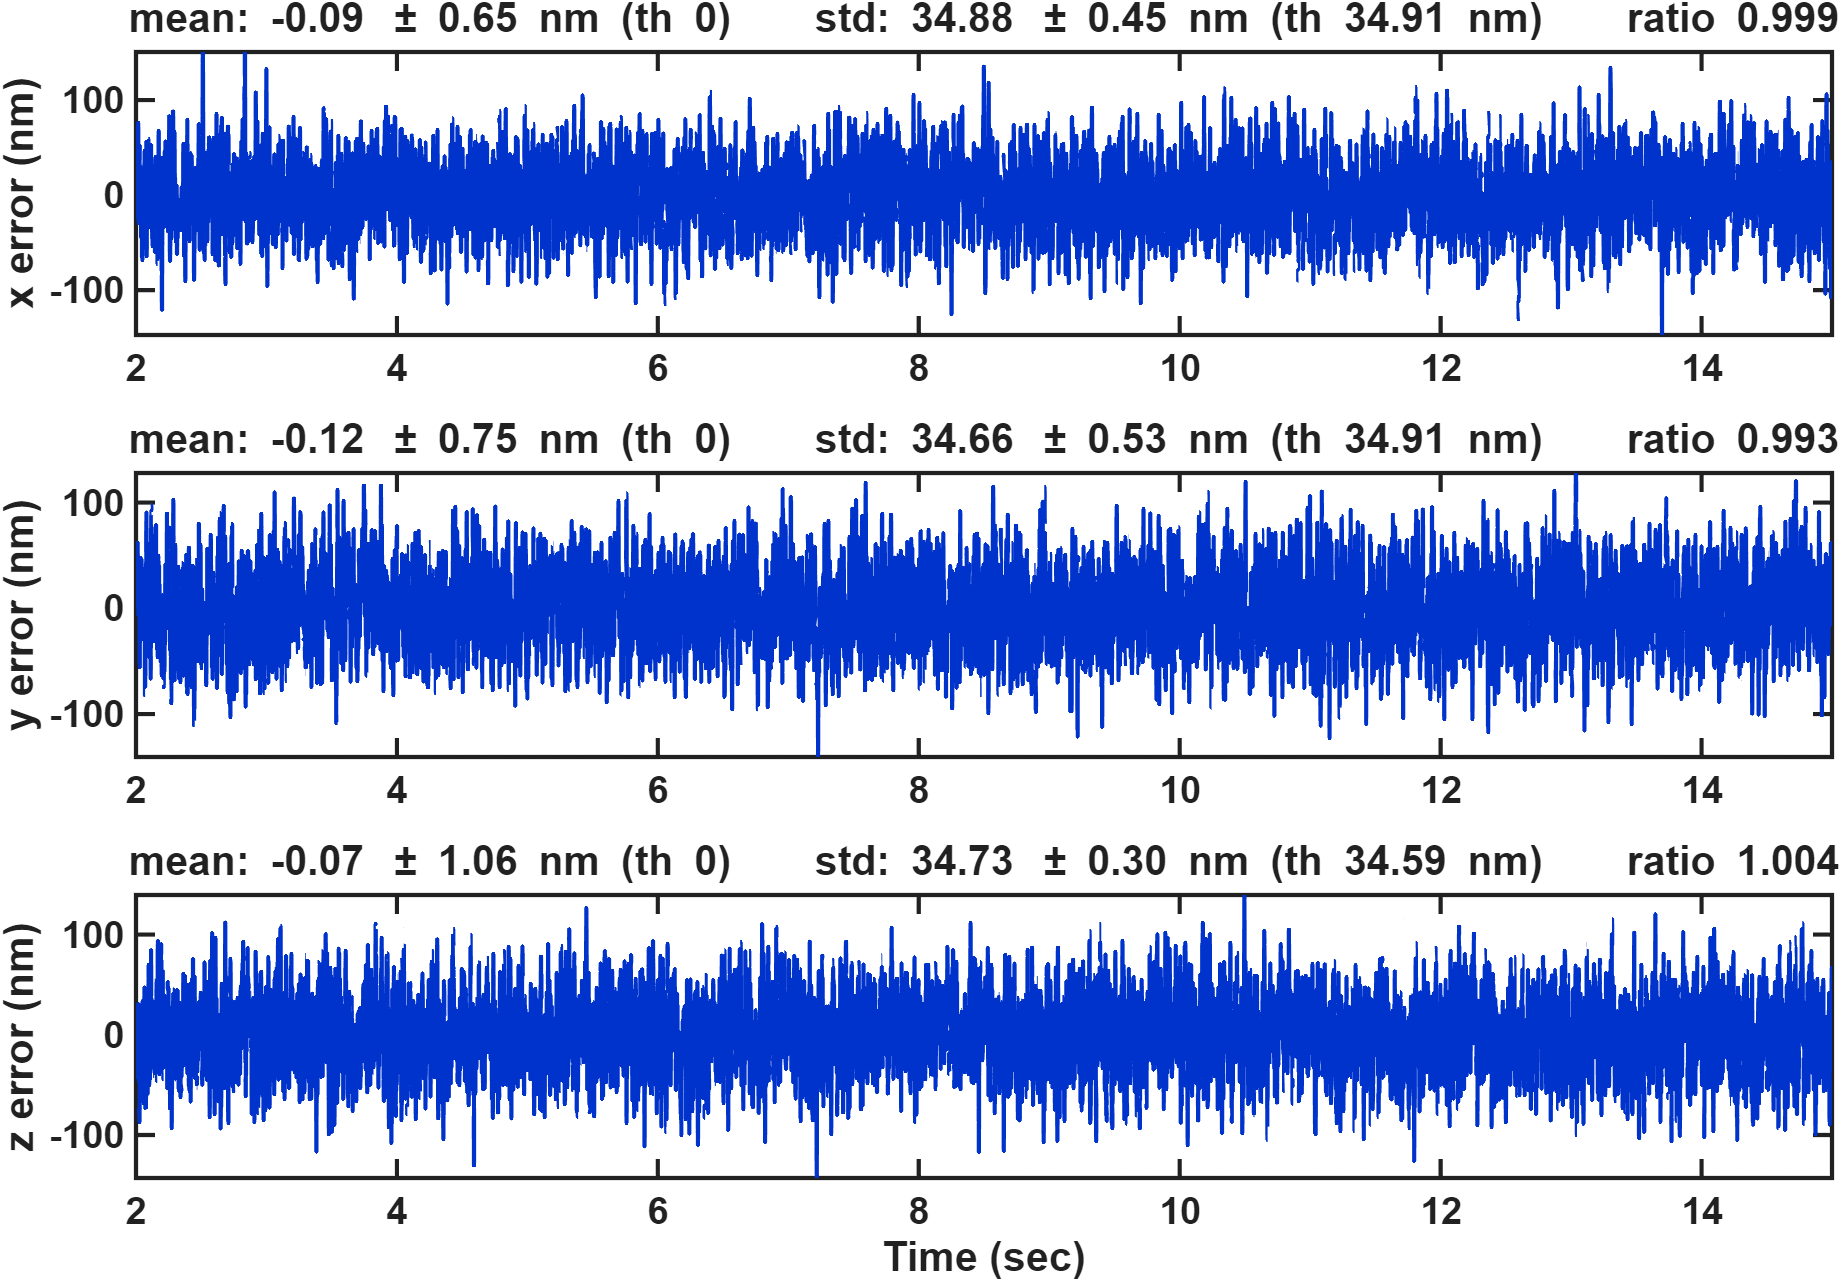
\includegraphics[width=0.92\textwidth]{fig_qr_h50_tracking_std.png}
\caption{Tracking error per axis ($h = 50\,\mu$m).}
\end{figure}

\clearpage
\begin{figure}[p]
\centering
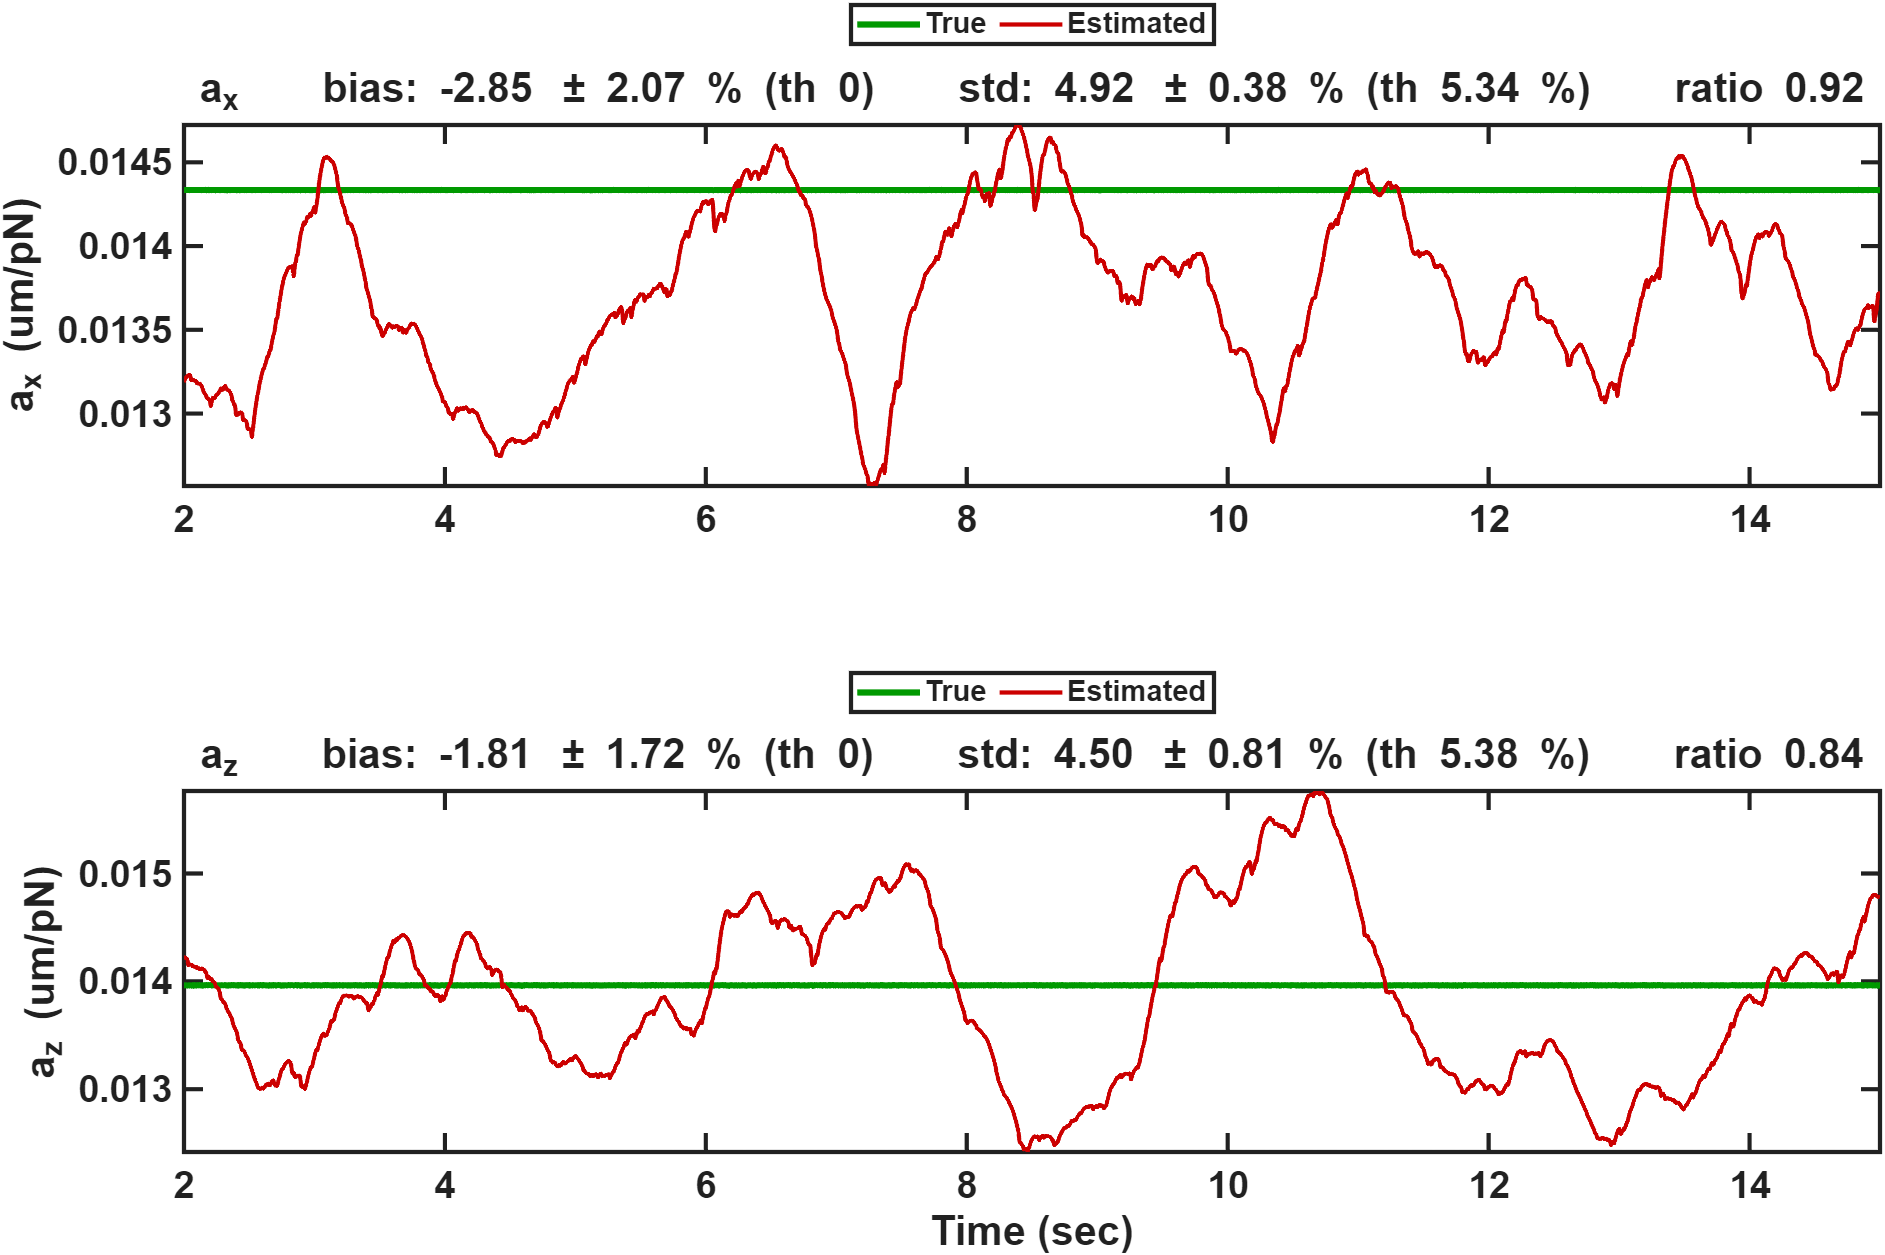
\includegraphics[width=0.92\textwidth]{fig_qr_h50_ahat_std.png}
\caption{Motion-gain estimation ($h = 50\,\mu$m).}
\end{figure}
=======
\subsection*{6.4\quad Bias factor (boxed)}

Substitute 6.3 into 6.1:
\begin{equation}
\boxed{\;\beta(\lc, a_{prd}) \;=\; 1 \;-\; \frac{a_{prd}}{2 - a_{prd}}\,\Bigl[\,1 + 2\sum_{m=1}^{\infty}\rho(m)(1{-}a_{prd})^{m}\,\Bigr]\;}
\end{equation}
The bracket $\bigl[\,1 + 2\sum_{m\geq 1}\rho(m)(1{-}a_{prd})^{m}\,\bigr]$ is the
\emph{autocorrelation amplification}: equals $1$ for white $\delta x_{mr}$,
$>\!1$ for positively-correlated (the typical closed-loop case).

In practice the sum is truncated at $m_{\max}\!=\!100$; with $a_{prd}\!=\!0.05$,
the residual $(1{-}a_{prd})^{m_{\max}}\!\approx\!0.006$ lies below numerical noise.

\subsection*{6.5\quad Numerical}

At $\lc = 0.7$, $a_{prd} = 0.05$:
\begin{align*}
\beta_{\mathrm{white}} &\;\equiv\; \frac{2 - 2 a_{prd}}{2 - a_{prd}} \;=\; 0.9744
  &&\text{(white reference; bracket}=1) \\[2pt]
\beta &\;=\; 0.9069
  &&\text{(closed-loop; bracket}\!\approx\!3.6) \\[2pt]
\text{bias amplification} &\;=\; \frac{1 - \beta}{1 - \beta_{\mathrm{white}}} \;\approx\; 3.6\times
\end{align*}

\subsection*{6.6\quad Bias-corrected estimator}

Section 2's estimator output satisfies
\[
\mathrm{E}\!\bigl[\,\sigma^{2}_{\delta x_{mr}}\,\bigr]
  \;=\; \beta\cdot\mathrm{Var}(\delta x_{mr})
  \;=\; \beta\,\bigl(C_{\mathrm{dpmr}}\cdot 4\kB T\,a_x + C_{n}\,\sigma^{2}_n\bigr).
\]
Inverting for $a_x$: first unbias $\sigma^{2}_{\delta x_{mr}}$ by $\beta$,
then apply Section 2's boxed formula:
\begin{equation}
\boxed{\;a_{xm}[k] \;=\; \frac{\sigma^{2}_{\delta x_{mr}}[k]/\beta \,-\, C_{n}\,\sigma^{2}_n}
                                   {C_{\mathrm{dpmr}}\cdot 4\kB T}\;}
\end{equation}
$\beta(\lc, a_{prd})$ is precomputed offline as a 2-D lookup table; runtime cost zero.
>>>>>>> test/qr-paper-reference

\end{document}
